\documentclass[titlepage, 12pt]{article}
\usepackage[utf8]{inputenc}
\usepackage{multirow}
\usepackage{graphicx}
\usepackage[english,serbian]{babel}

\title{Luis fon An\\ \small{Seminarski rad u okviru kursa\\Tehničko i naučno pisanje\\ Matematički fakultet}}
\author{Aleksandar Šmigić \\ mi19028@alas.matf.bg.ac.rs \and Andrijana Milić \\ mi18186@alas.matf.bg.ac.rs \and Miloš Petričković \\ mi18055@alas.matf.bg.ac.rs \and Nikola Milutinović \\ mi18202@alas.matf.bg.ac.rs}
\date{Novembar 2019}

\begin{document}

\maketitle

\tableofcontents
\newpage
\section{Uvod}

{\renewcommand{\arraystretch}{1.2}}
\begin{tabular}{|c|c|c|}
\hline
\multicolumn{2}{|c|}{\Large{Luis fon An}}\\[4px]
\hline
\multicolumn{2}{|c|}{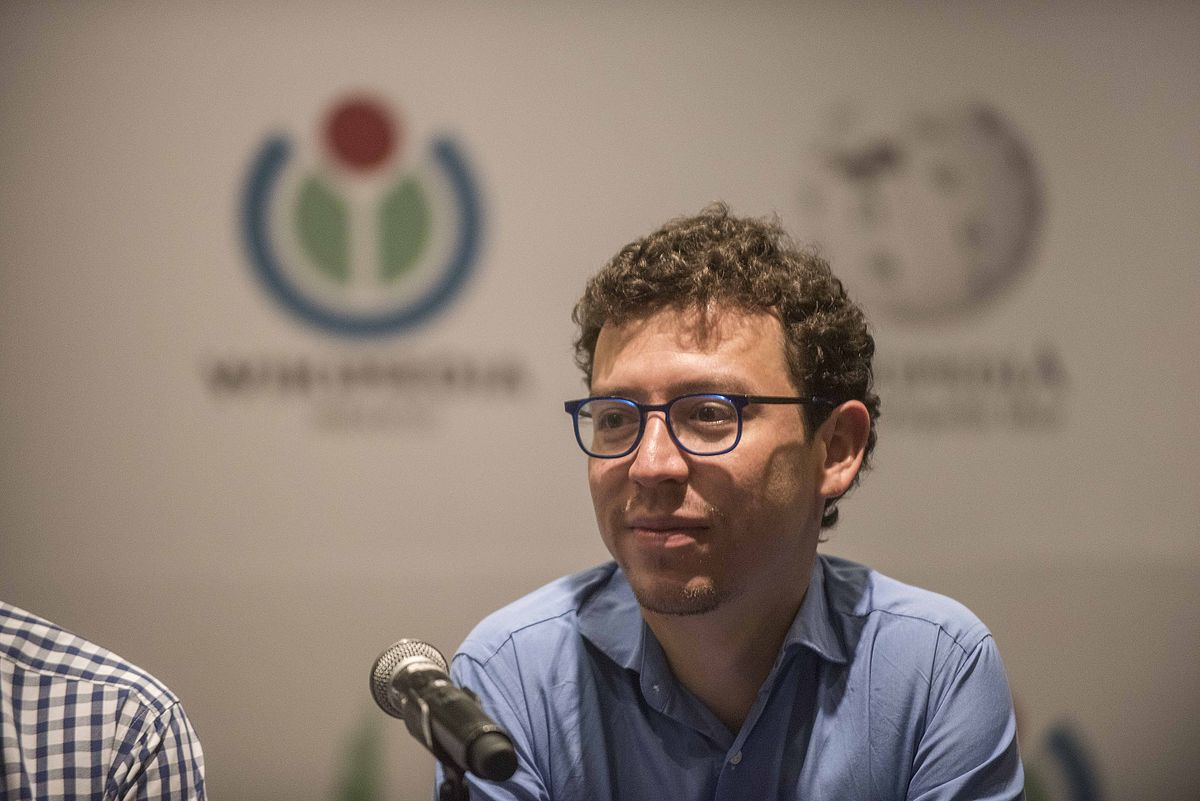
\includegraphics[width=320px,height=216px]{Luis_von_Ahn.jpg}}\\

\hline
Datum rođenja & 19.8.1955. \\
\hline
Mesto rođenja & Gvatemala, Gvatemala\\
\hline
Prebivalište & Berkli(Kalifornija)\\
\hline
\multirow{2}{*}{Institucije}&Univerzitet Karnegi Melon\\
& Univerzitet Djuk \\
\hline 
\multirow{3}{*}{Poznat po} & CAPTCHA \\
& reCAPTCHA \\ & Duolingo \\
\hline
\multirow{2}{*}{Nagrade} & MacArthur Fellowship (2006) \\
 & TR35 (2007)
\\
\hline
\end{tabular}

\vspace{20px}

Luis fon An, rođen 19. avgusta 1978. je gvatemalski preduzetnik i profesor konsultant na odseku za računarstvo na univerzitetu Karnegi Melon u Pitsburgu u Pensilvaniji.[1] Poznat je kao jedan od začetnika crowdsourcing-a. On je osnivač kompanije reKapča (engl. reCAPTCHA), koja je prodata Guglu 2009. godine, [2] i jedan od osnivača i glavni izvršni direktor Duolinga, popularne platforme za učenje jezika. 

\end{document}
